In this section we empirically demonstrate that our CASH mechanism can be used to significantly reduce the fraction of accounts that an offline adversary could compromise. We implemented Algorithm \ref{alg:HeuristicAlg2} in C\# using Gurobi as our LP solver, and analyzed CASH using two real-world password distributions . The first distribution is based on data from the RockYou password breach ( million passwords) and the second is based on password frequency data from Yahoo! users (representing  million passwords). The later dataset was not the result of a security breach. Instead, Yahoo! gave Bonneau~\cite{bonneau2012science} permission to collect and analyze password frequency data in a carefully controlled environment. Yahoo! recently allowed Blocki et al.~\cite{blocki2016differentially} to use a differentially private~\cite{dwork2006calibrating} algorithm to publish this data. Thus, the password frequency data in this data set has been perturbed slightly.  Blocki et al.~\cite{blocki2016differentially} also showed that with high probability the L1 error introduced by their algorithm would be minimal. 


In each of our experiments we fix the password correctness rate  and the maximum amortized server cost  before using Algorithm \ref{alg:HeuristicAlg2} to find a CASH parameters  and  subject to the appropriate constraints on the amortized server costs. 

We compare the  of cracked passwords under three different scenarios: 
\begin{itemize}
\item (Deterministic Key-Stretching) The authentication server selects a hash function   with cost parameter   (achieved through traditional deterministic key-stretching techniques). The rational value  adversary will crack each password with probability  (eq \ref{eq:PAdvDet}).   
\item (Uniform-CASH) The authentication server uses CASH with the uniform distribution. He sets  according to eq \ref{eq:kUnifCash}
to ensure that his amortized costs are at most . A rational value  adversary will crack each password with probability . 

\item (CASH) Given an estimate  of the adversary's budget we used Algorithm \ref{alg:HeuristicAlg2} to optimize the CASH parameters  and  subject to the constraint that the amortized server cost is at most  when users enter the wrong password with probability . We fixed the parameters , and we set , , , , ,  , , , , , . Thus, Algorithm \ref{alg:HeuristicAlg2} computes the optimal distribution against a threshold  adversary for each , and selects the best distribution  against a value  adversary.   will denote the fraction of cracked passwords when the true value is . When the adversary's true value is ,   will denote the fraction of cracked passwords.  
\end{itemize}

Our results indicate that an authentication server could significantly reduce the fraction of compromised passwords in an offline attack by adopting our optimal CASH mechanism instead of deterministic key-stretching or uniform-CASH. These results held robustly for both the RockYou and Yahoo! password distributions.






\subsubsection{Password Datasets} \label{subsubsec:RockYou} We use two password frequency datasets, RockYou and Yahoo!, to analyze our CASH mechanism. The RockYou dataset contains passwords from  million RockYou users, and the Yahoo! dataset contains data from  million Yahoo! users. We used frequency data from each of these datasets to obtain an empirical password distribution  over . 

The RockYou dataset is based on actual user passwords which were leaked during the infamous RockYou security breach (RockYou had been storing these passwords in the clear). The total number of unique passwords in the dataset was  million. Approximately,  million of these passwords were unique to one RockYou user. The other  million passwords were used by multiple users. The most popular password ( `123456') was shared by  million RockYou users (). RockYou did not impose strict password restrictions on its users (e.g. users were allowed to select passwords consisting of only lowercase letters or only numbers). 

We also used (perturbed) password frequency data from a dataset of  million Yahoo! passwords. See~\cite{bonneau2012science} for more details about how this data was collected and see~\cite{blocki2016differentially} for more details about how the frequency data was perturbed to satisfy the rigorous notion of differentially privacy~\cite{dwork2006calibrating}. Blocki et al.~\cite{blocki2016differentially} proved that with high probability the L1 distortion of the perturbed frequency data is bounded by , where the privacy parameter was set to  when the Yahoo! dataset was published. Thus, the perturbed dataset will also still give us a good estimate of the empirical password distribution.  

\cut{
\subsubsection{Comparing Defenses}
Given fixed values  and  it is critically important to make a fair comparison between the different defenses that the authentication server might adopt. If the authentication server adopts a deterministic key-stretching algorithm  then he can afford to set  so that his average cost per authentication is . In this case the adversary can guess  passwords (to simplify presentation we assume that  divides ) so we have 
Similarly, if the authentication server adopts the uniform-CASH strategy with  then he can afford to set 

so that his average cost per login is at most . 
In this case we will have 
because the adversary's optimal strategy is to spend all of his budget guessing the  most popular passwords. Finally, if the authentication server adopts our CASH mechanism then he will run algorithm \ref{alg:HeuristicAlg} with the fixed values  to obtain . The algorithm is guaranteed to find a solution in which the average cost at most . In this case the adversary's success rate is 



\subsubsection{Parameter Selection} \label{subsubsec:ParameterTuning}
In each experiment we fixed the ratio , the ratio between the work that the offline adversary is willing to do and the work that a legitimate authentication server needs to do on average. If the authentication server uses  rounds of deterministic key-stretching then  denotes the total number of password guesses that the offline adversary can try. In our experiments, we considered the following range of values for this ratio : .  We expect that the adversary's success rate   will increase as this ratio increases --- a server that is willing to do more work on average during authentication can better protect its users. 

When selecting  and  we need to ensure that . In general, we get more flexibility in our optimization problem by selecting  large and then selecting . However, the optimization problem becomes harder to solve as  increases. Thus, we fixed  when optimizing CASH while allowing  to vary because we could not find any noticeable improvement in obtained CASH solutions for . We used our CASH optimization algorithm to optimize the value and  as well as . }


\subsection{Results}
Our first set of experimental results are shown in Figures \ref{fig:YahooResults1} and \ref{fig:RockYouResults1}. These plots were computed under the assumption that  (users always enter their passwords correctly), and that  (the defender knows the exact adversary value). The results show that for some (higher) adversary values our non-uniform CASH distributions improves significantly on the cost-equivalent versions of uniform CASH ( reduction in cracked passwords) and deterministic key-stretching ( reduction in cracked passwords).\footnote{We note that we would expect to see relatively high adversary  values  in the offline setting because  will typically be quite small (e.g., 10^{-6}\alpha = 0.9\alpha=0.95\hat{v} \neq v\hat{v}\tilde{p}\tilde{p}\tilde{p}\tilde{p}\alpha=1\frac{v}{C_{max}}\%\PAdvCASH{v}{v}{C_{max}}\PAdvUnif{v}{C_{max}}\PAdvDet{v}{C_{max}}--\alpha = 1\alpha=1\frac{v}{C_{max}}\frac{v}{C_{max}}\%\PAdvCASH{v}{v}{C_{max}}\PAdvUnif{v}{C_{max}}\PAdvDet{v}{C_{max}}--\alpha = 1\alpha=0.95\frac{v}{C_{max}}\%\PAdvCASH{v}{v}{C_{max}}\PAdvUnif{v}{C_{max}}\PAdvDet{v}{C_{max}}--\hat{v}\neq v\alpha=0.95, \hat{v} = C_{max}\times 10^4\frac{v}{C_{max}}\PAdvCASH{v}{\hat{v}}{C_{max}}\PAdvUnif{v}{C_{max}}\PAdvDet{v}{C_{max}}--v = \hat{v}\hat{v}\neq v\alpha=0.95, \hat{v} = 7\times C_{max} \times 10^7\frac{v}{C_{max}}\PAdvCASH{v}{\hat{v}}{C_{max}}\PAdvUnif{v}{C_{max}}\PAdvDet{v}{C_{max}}--v = \hat{v}\alpha=0.95\frac{v}{C_{max}}\%\PAdvCASH{v}{v}{C_{max}}\PAdvUnif{v}{C_{max}}\PAdvDet{v}{C_{max}}--\hat{v} \neq v\alpha=0.95, \hat{v} = C_{max}\times 10^4\frac{v}{C_{max}}\PAdvCASH{v}{\hat{v}}{C_{max}}\PAdvUnif{v}{C_{max}}\PAdvDet{v}{C_{max}}--v = \hat{v}\hat{v} \neq v\alpha=0.95, \hat{v} = 7\times C_{max} \times 10^7\frac{v}{C_{max}}\PAdvCASH{v}{\hat{v}}{C_{max}}\PAdvUnif{v}{C_{max}}\PAdvDet{v}{C_{max}}--v = \hat{v}\alpha=0.95\alpha \in \{0.9,0.95,1\}\alpha\alpha \rightarrow 0\alpha\alpha\alpha = 0.9\alpha=0.951-\alpha\alphav\hat{v}v\hat{v}\tilde{p}\mathbf{Cost}\left(\mathbf{H}\right)\--30\ might be a reasonable upper bound on the adversary's value for a cracked password (measured in \# of computations of ). We would also strongly advocate for the use of memory hard functions instead of hash iteration to increase  effectively (see discussion in Section \ref{subsec:Traditional}). 


 \begin{figure}[!t]
\subfloat[Yahoo Dataset.]{
      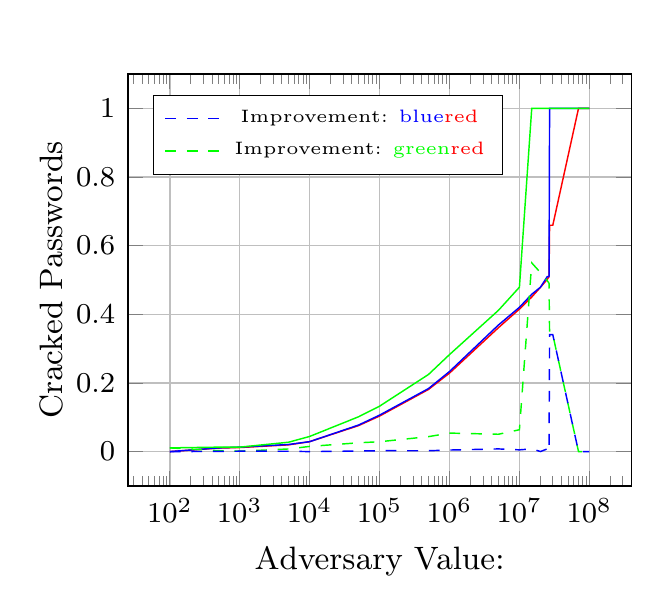
\begin{tikzpicture}[scale=1.3]  
   \begin{semilogxaxis}[
    title style={align=center},
    title={ {\small  }},
    xlabel={Adversary Value: },
    ylabel={ Cracked Passwords},
    ylabel shift = -3pt,
grid=major,
    small,
    cycle list = {{red, mark=none}, {blue, mark=none}, {green, mark=none},{green, dashed, mark=none}, {blue, dashed, mark=none},  {blue, dashed, mark=none}, {red, dashed, mark=none},{brown, dashed, mark=none} },
    legend style = {font=\tiny, at={(.05,.95)}, anchor=north west},
    legend entries = { , , , Improvement: \textcolor{blue}{blue}\textcolor{red}{red}, Improvement: \textcolor{green}{green}\textcolor{red}{red}}
   ] 

    \addlegendimage{no markers, red, mark=square*}
    \addlegendimage{no markers, blue, mark=square*}
    \addlegendimage{no markers, green, mark=square*}
    \addlegendimage{no markers, dashed, blue}
    \addlegendimage{no markers, dashed, green}
\addplot coordinates {  (100,0)  (500,0.0103650003300184)  (1000,0.0118193070978086)  (5000,0.0196537617974582)  (10000,0.0289970884688705)  (50000,0.0757213976299667)  (100000,0.103595972530575)  (500000,0.181006843045768)  (1000000,0.228656981329561)  (5000000,0.360821094325625)  (10000000,0.415177925518485)  (15000000,0.450283451843314)  (20000000,0.47863343472216)  (25000000,0.501829516819531)  (26500000,0.509750280863969)  (27000000,0.659338193697864)  (27500000,0.659338193697864)  (28000000,0.659338193697864)  (29000000,0.659338193697864)  (30000000,0.659338193697864)  (70000000,0.999999999999979)  (100000000,0.999999999999979)  };
\addplot coordinates {  (100,0)  (500,0.0108687224894377)  (1000,0.0130192581998815)  (5000,0.0207614032035197)  (10000,0.0289970884688704)  (50000,0.0773727496772537)  (100000,0.106225338769438)  (500000,0.183571148129509)  (1000000,0.233240940214472)  (5000000,0.368658241037976)  (10000000,0.420317345392629)  (15000000,0.45834913690049)  (20000000,0.478853387778074)  (25000000,0.50975028086399)  (26500000,0.50975028086399)  (27000000,1)  (27500000,1)  (28000000,1)  (29000000,1)  (30000000,1)  (70000000,1)  (100000000,1)  };
\addplot coordinates {  (100,0.0108687224894377)  (500,0.0130192581998815)  (1000,0.0130192581998815)  (5000,0.0273838584095427)  (10000,0.0441510096695537)  (50000,0.101412040578669)  (100000,0.132372669808665)  (500000,0.224601121331902)  (1000000,0.282624504055384)  (5000000,0.411368138539665)  (10000000,0.478853387778074)  (15000000,1)  (20000000,1)  (25000000,1)  (26500000,1)  (27000000,1)  (27500000,1)  (28000000,1)  (29000000,1)  (30000000,1)  (70000000,1)  (100000000,1)  };
\addplot coordinates {  (100,0.0108687224894377)  (500,0.00265425786986305)  (1000,0.00119995110207291)  (5000,0.00773009661208442)  (10000,0.0151539212006832)  (50000,0.025690642948702)  (100000,0.0287766972780896)  (500000,0.0435942782861336)  (1000000,0.053967522725823)  (5000000,0.0505470442140399)  (10000000,0.0636754622595894)  (15000000,0.549716548156686)  (20000000,0.52136656527784)  (25000000,0.498170483180469)  (26500000,0.490249719136031)  (27000000,0.340661806302136)  (27500000,0.340661806302136)  (28000000,0.340661806302136)  (29000000,0.340661806302136)  (30000000,0.340661806302136)  (70000000,2.14273043752655E-14)  (100000000,2.14273043752655E-14)  };
\addplot coordinates {  (100,0)  (500,0.000503722159419252)  (1000,0.00119995110207291)  (5000,0.00110764140606149)  (10000,-1.49186218934005E-16)  (50000,0.00165135204728702)  (100000,0.00262936623886303)  (500000,0.00256430508374061)  (1000000,0.00458395888491178)  (5000000,0.00783714671235103)  (10000000,0.00513941987414457)  (15000000,0.0080656850571757)  (20000000,0.000219953055913658)  (25000000,0.00792076404445874)  (26500000,2.1094237467878E-14)  (27000000,0.340661806302136)  (27500000,0.340661806302136)  (28000000,0.340661806302136)  (29000000,0.340661806302136)  (30000000,0.340661806302136)  (70000000,2.14273043752655E-14)  (100000000,2.14273043752655E-14)  };


   \end{semilogxaxis} 
  \end{tikzpicture}
  
\label{fig:YahooResults90}}
\subfloat[RockYou Dataset.]{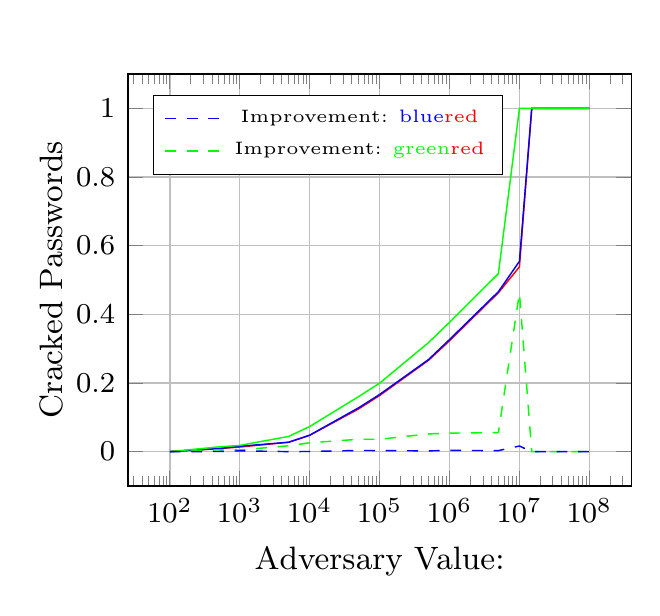
\begin{tikzpicture}[scale=1.3]  
   \begin{semilogxaxis}[
    title style={align=center},
    title={ {\small  }},
    xlabel={Adversary Value: },
    ylabel={ Cracked Passwords},
    ylabel shift = -3pt,
grid=major,
    small,
    cycle list = {{red, mark=none}, {blue, mark=none}, {green, mark=none},{green, dashed, mark=none}, {blue, dashed, mark=none},  {blue, dashed, mark=none}, {red, dashed, mark=none},{brown, dashed, mark=none} },
    legend style = {font=\tiny, at={(.05,.95)}, anchor=north west},
    legend entries = { , , , Improvement: \textcolor{blue}{blue}\textcolor{red}{red}, Improvement: \textcolor{green}{green}\textcolor{red}{red}}
   ] 

    \addlegendimage{no markers, red, mark=square*}
    \addlegendimage{no markers, blue, mark=square*}
    \addlegendimage{no markers, green, mark=square*}
    \addlegendimage{no markers, dashed, blue}
    \addlegendimage{no markers, dashed, green}
\addplot coordinates {  (100,0)  (500,0.00859451942407725)  (1000,0.0133447400377569)  (5000,0.0272760303315716)  (10000,0.0474032707627518)  (50000,0.124170424428517)  (100000,0.163294928646465)  (500000,0.265801301128427)  (1000000,0.322799966527542)  (5000000,0.462803564928199)  (10000000,0.538000264865568)  (15000000,0.999999999999978)  (20000000,0.999999999999978)  (25000000,0.999999999999978)  (26500000,0.999999999999978)  (27000000,0.999999999999978)  (27500000,0.999999999999978)  (28000000,0.999999999999978)  (29000000,0.999999999999978)  (30000000,0.999999999999978)  (70000000,0.999999999999978)  (100000000,0.999999999999978)  };
\addplot coordinates {  (100,0)  (500,0.00891714075850031)  (1000,0.0155215770827253)  (5000,0.0272760303315717)  (10000,0.0478123623225905)  (50000,0.127514539286531)  (100000,0.166347957457673)  (500000,0.267932308139264)  (1000000,0.326354365380677)  (5000000,0.465731506185799)  (10000000,0.55428368364662)  (15000000,1)  (20000000,1)  (25000000,1)  (26500000,1)  (27000000,1)  (27500000,1)  (28000000,1)  (29000000,1)  (30000000,1)  (70000000,1)  (100000000,1)  };
\addplot coordinates {  (100,0)  (500,0.0136977788934083)  (1000,0.0180747779954648)  (5000,0.0441965417827129)  (10000,0.0730608733055595)  (50000,0.160089926850547)  (100000,0.199287847017616)  (500000,0.317302545367371)  (1000000,0.376634078642379)  (5000000,0.518411276766697)  (10000000,1)  (15000000,1)  (20000000,1)  (25000000,1)  (26500000,1)  (27000000,1)  (27500000,1)  (28000000,1)  (29000000,1)  (30000000,1)  (70000000,1)  (100000000,1)  };
\addplot coordinates {  (100,0)  (500,0.00510325946933101)  (1000,0.00473003795770787)  (5000,0.0169205114511413)  (10000,0.0256576025428077)  (50000,0.0359195024220297)  (100000,0.0359929183711517)  (500000,0.0515012442389441)  (1000000,0.0538341121148372)  (5000000,0.0556077118384979)  (10000000,0.461999735134432)  (15000000,2.22044604925031E-14)  (20000000,2.22044604925031E-14)  (25000000,2.22044604925031E-14)  (26500000,2.22044604925031E-14)  (27000000,2.22044604925031E-14)  (27500000,2.22044604925031E-14)  (28000000,2.22044604925031E-14)  (29000000,2.22044604925031E-14)  (30000000,2.22044604925031E-14)  (70000000,2.22044604925031E-14)  (100000000,2.22044604925031E-14)  };
\addplot coordinates {  (100,0)  (500,0.000322621334423063)  (1000,0.00217683704496837)  (5000,8.32667268468867E-17)  (10000,0.000409091559838717)  (50000,0.00334411485801335)  (100000,0.00305302881120795)  (500000,0.0021310070108374)  (1000000,0.00355439885313574)  (5000000,0.00292794125760004)  (10000000,0.0162834187810521)  (15000000,2.22044604925031E-14)  (20000000,2.22044604925031E-14)  (25000000,2.22044604925031E-14)  (26500000,2.22044604925031E-14)  (27000000,2.22044604925031E-14)  (27500000,2.22044604925031E-14)  (28000000,2.22044604925031E-14)  (29000000,2.22044604925031E-14)  (30000000,2.22044604925031E-14)  (70000000,2.22044604925031E-14)  (100000000,2.22044604925031E-14)  };


   \end{semilogxaxis} 
  \end{tikzpicture}
  
\label{fig:RockYouResults90}}
\centering
\caption{.}
\end{figure}

\paragraph{Obtaining an Empirical Password Distribution} We remark that the specific CASH distributions we computed for the RockYou and Yahoo! datasets might not be optimal in other application settings because the underlying password distribution may vary across different contexts. For example, users might be more motivated to pick strong passwords for higher value accounts (e.g., bank accounts). Similarly, some organizations choose to restrict the passwords that a user may select (e.g., requiring upper and lower case letters). While these restrictions do not always result in stronger passwords~\cite{usability:compositionPolicies}, they can alter the underlying password distribution~\cite{blockiPasswordComposition}. While the underlying distribution may vary from context to context, we note that an authentication server could always follow the framework of Bonneau~\cite{bonneau2012science} and Blocki et al.~\cite{blocki2016differentially} to securely approximate the password distribution  of its own users. 

If an organization remains highly uncertain about value  of a cracked password or about the empirical password distribution  then it may be prudent to adopt the uniform-CASH mechanism (e.g., \cite{manber1996simple}), which {\em always } performs at least as well as the traditional key-stretching approach.

\subsubsection{Experimental Limitations} \label{subsubsec:Limitations}
We remark that values of  that we compute in our experiments may be less realistic for larger values of  (e.g., ). The reason is that , our empirical estimate of the probability of password , will be too high for many of our unique passwords in the dataset. For example, consider a dedicated user who memorizes a truly random  character string of upper and lower case letters. The true probability that any individual password guess matches the user's password would be at most . However, if that password occurred in the RockYou dataset then our empirical estimate of this probability would be at least . Developing improved techniques for estimating the true likelihood of unique password in a password frequency dataset is an important research direction.
